\chapter{Simulation and Validation}\label{sec: Simulation Framework}
\textbf{TEXTTTTTTTT}
\section{Simulation Methods}\label{sec: simulation methods}
Observations are simulated to test the effectiveness of \gls{x-bap}. A fiducial model is defined, with which various aspects are varied to test what the limitations of this method are. The simulated images are 128 by 128 pixels. This pixel scale is chosen as this is the same pixel scale used later for the flux measurements in the \gls{mer} observations. Furthermore, as the Fast Fourier Transform relies on splitting arrays into even and odd terms, it performs best when the arrays have sizes that are powers of two.  An elliptical Gaussian is chosen for the galaxy's intrinsic image, with standard deviations of five pixels along the y-axis and ten pixels along the x-axis,

\begin{equation}
    I(x,y) \propto \exp\left(-\frac{1}{2}\left(\frac{x^2}{10^2}+\frac{y^2}{5^2}\right)\right),
\end{equation}
where the origin is in the center of the image.
The sum of the pixel values of this intrinsic image $I$ of the galaxy is 1000. This intrinsic image is then convolved with a normalized Gaussian \gls{psf} $P$ with a standard deviation of 3 pixels,

\begin{equation}
    P(x,y) \propto \exp\left(-\left(\frac{x^2+y^2}{3^2}\right)\right).
\end{equation}
The \gls{psf} is normalized such that the pixel values sum to one.
The fiducial weight function is a normalized Gaussian with a standard deviation of eight pixels. The noise $N$ in the simulated image is drawn from a Gaussian distribution with mean zero and variance 0.01. The resulting observation is the combination of the \gls{psf}, intrinsic image, and the noise
\begin{equation}
    O = P\otimes I + N.
\end{equation}

\begin{figure}[H]
    \centering
    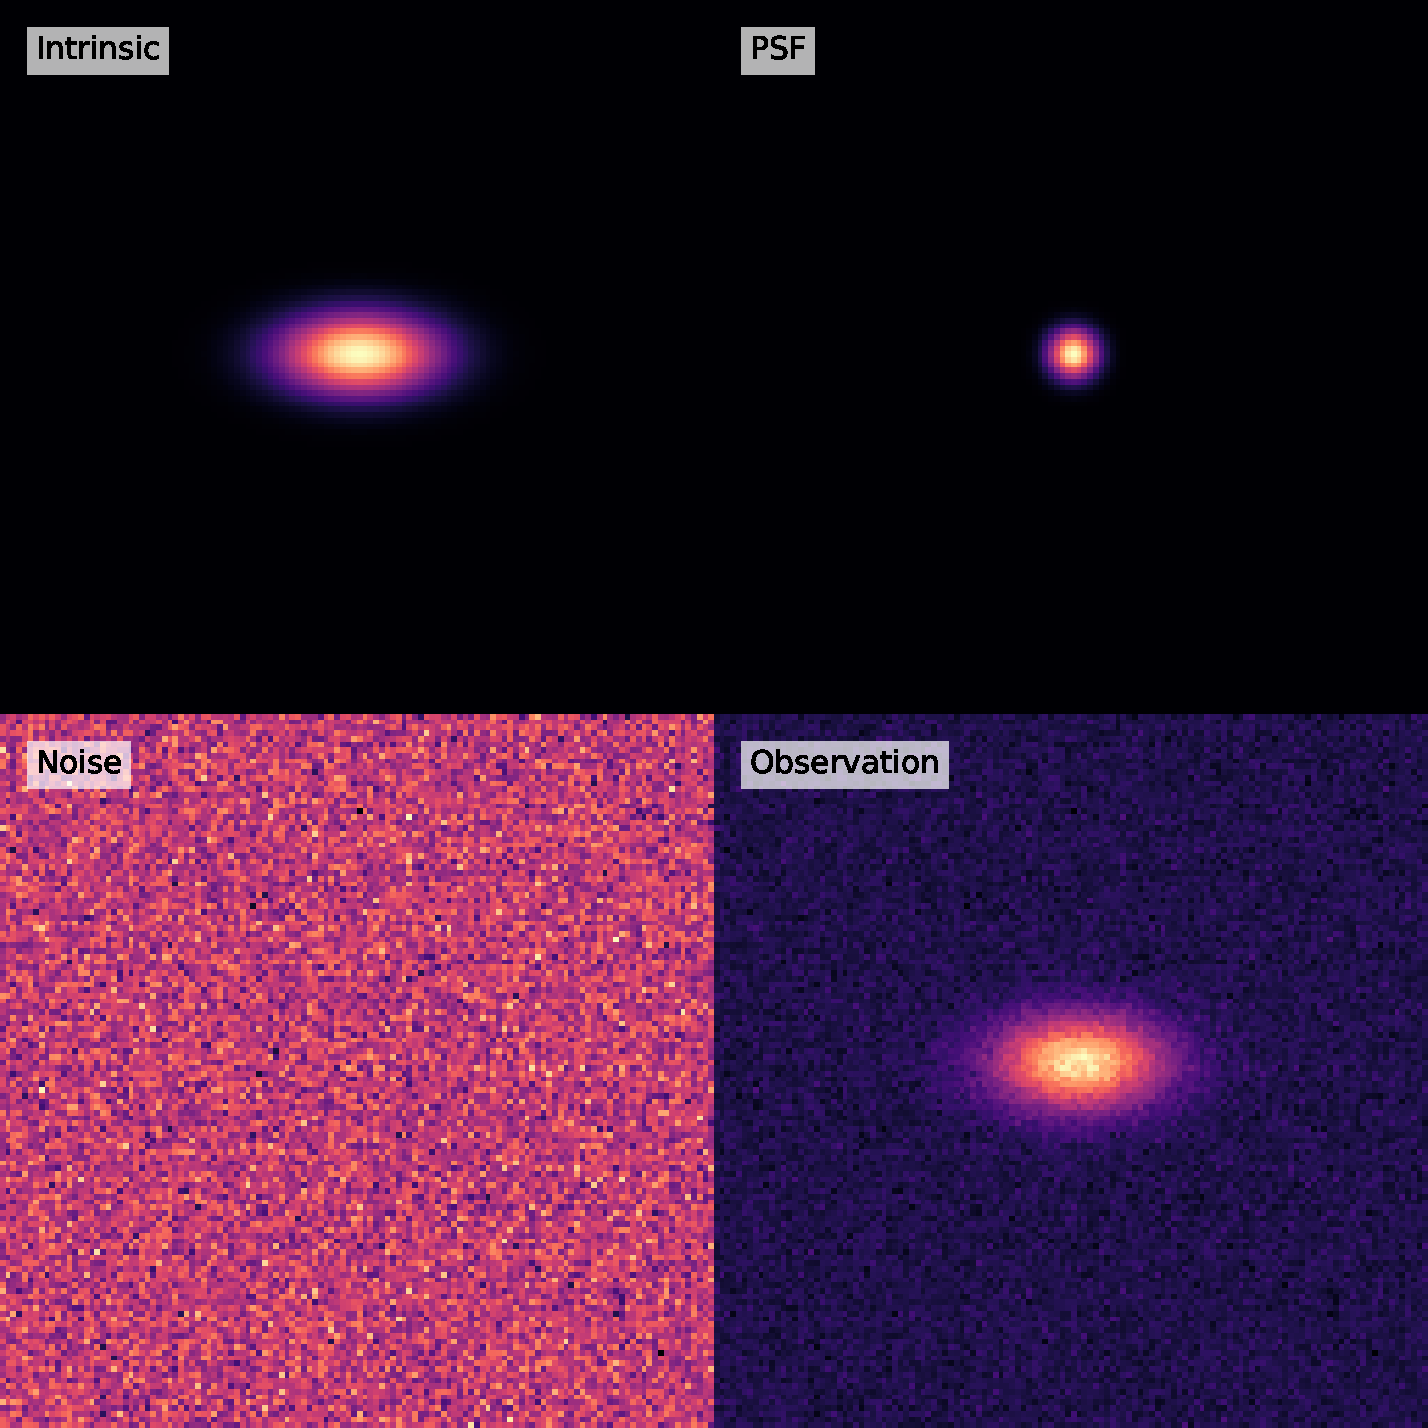
\includegraphics[width=0.6\linewidth]{results/figures/simulation/fiducial_model.pdf}
    \caption{The elliptical Gaussian intrinsic image of the galaxy  (top left), the \gls{psf} (top right), and the noise (bottom left) are combined to form the fiducial observation (bottom right).}
    \label{fig: fiducial model}
\end{figure}
\noindent Next, each component of the fiducial model is varied individually to investigate the consequences of each part on the measured flux and the estimated error.  


\subsection{Flux Accuracy}\label{subsec: flux accuracy}

The flux determined from the pre-seeing image with the pre-seeing weight

\begin{equation}
    F_\mathrm{True} = \int dxdy I(x,y) \tilde{W}_\mathrm{A}(x,y)
\end{equation}
is used compared to the aperture flux measured with the deconvolved weight and the observed image with noise

\begin{equation}
    F_\mathrm{Measured} = \int dxdy O(x,y) W_\mathrm{A}(x,y).
\end{equation}
The fractional error in the flux is used to gain insight into where \gls{x-bap} works and, more importantly, where it fails. The flux is measured at different points in the image, which means that the same weight function is used but the center of the weight function is shifted to different points \textbf{ILLUSTRATION?}. Next, the aperture flux is measured for different combinations of \gls{psf} size and size of the weight function, where both are Gaussian. The fractional error can be calculated using

\begin{equation}
    \epsilon_F=\frac{F_\mathrm{Measured}- F_\mathrm{True}}{F_\mathrm{True}}.
\end{equation}
The fractional error is preferred over an absolute error as the measured flux depends on the size of the weight function. The fractional error corrects for the difference in scale involved and allows for an easier evaluation of the accuracy of the \gls{x-bap} method.

\subsection{Error Accuracy}
To assess the accuracy of the error, different noise realizations are generated, and the flux $F_i$ and error $\sigma_i$ are computed for each realization. The standard deviation of the flux values is taken as the true standard deviation, $\sigma_\mathrm{True}=\mathrm{std}(F_i)$. The mean of the measured errors $\sigma_\mathrm{Measured}=\mathrm{mean}(\sigma_i)$ is used to compute the relative error on the error of the flux
\begin{equation}
    \epsilon_\sigma = \frac{\sigma_\mathrm{Measured}- \sigma_\mathrm{True}}{\sigma_\mathrm{True}}.
\end{equation}
This is repeated for different combinations of weight and \gls{psf} sizes in the same way as in \Cref{subsec: flux accuracy}.

Up until this point, the noise in the simulations was uncorrelated. However, in real observations, this is rarely the case. To simulate correlated noise, uncorrelated noise is convolved with a Gaussian with a scale parameter called 'noise scale'. There are two different methods to estimate the error on the aperture flux as discussed in \Cref{subsec: Noise Estimation from background Noise} and \Cref{subsec: Noise from RMS}. Both methods are tested for accuracy by generating 10,000 different noisy images for the simulation. For the method that only uses the background noise to estimate the error on the aperture flux (\Cref{subsec: Noise Estimation from background Noise}), only the simulated noise is provided to the algorithm. For the other method that also uses \gls{rms} (\Cref{subsec: Noise from RMS}), the simulated noise is used to get information about the correlation between pixels, and the \gls{rms} is a uniform image corresponding to the variance of the noise. \textbf{CORRELATED NOISE}
% The accuracy of the correlated noise also depends on the lag chosen in \autoref{eq: variance correlated}. This lag can be estimated from the local covariance matrix, where $L$ is chosen to center the matrix at the point where the absolute sum of its values exceeds 99\% of the sum of the absolute values of the full local covariance matrix.


\subsection{PSF Shape}

To test the method for robustness against variations in the \gls{psf} used for the deconvolution compared to the true \gls{psf}, the flux of the object is calculated using \glspl{psf} of different sizes and compared to the true value of the flux. In practice, it is impossible to perfectly model the \gls{psf} due to spatial variations, incomplete modeling etc. 


\subsection{Aperture Shape}

The shape of the weight function also influences what flux is measured and the \gls{snr} of that measurement. Different sizes of weight functions are tested on the fiducial image to get information on how the shape of the weight function influences the \gls{snr}. For this, elliptical Gaussian weight functions are used with different combinations of scale parameters on the x-axis and the y-axis. The choice of Gaussian weight functions is because their analytical Fourier transform is known and they are smooth functions, which result in a more stable deconvolution, unlike a top-hat function.

The \gls{x-bap} method is tested on simulated images as specified in \autoref{sec: Simulation Framework}. The results of these simulations are shown and discussed in this section.

\newpage
\section{Simulation Results}
After laying down the mathematical background for \gls{x-bap} in \Cref{ch: x-bap}, and setting up the simulation in \Cref{sec: simulation methods}, the results are shown in this section. 
\subsection{Deconvolution}\label{subsec: Deconvolution}

Before the \gls{x-bap} method can be applied, the deconvolution method must be tested to ensure it yields an accurate result. The deconvolution is stable when the weight is 'larger' than the \gls{psf}. In theory, this is straightforward to derive because both the \gls{psf} and weight function are approximately Gaussian, so comparing their scale factors yields a direct measure of their relative sizes. The convolution of two Gaussians yields a Gaussian with a variance equal to the sum of the variances of the original Gaussians. So the deconvolution of a weight function with a variance of $\sigma_\mathrm{weight}^2$ with a \gls{psf} with a variance of $\sigma_\mathrm{PSF}^2$ gives the deconvolved weight with a variance $\sigma^2_\mathrm{deconvolution}=\sigma^2_\mathrm{weight}-\sigma^2_\mathrm{PSF}$. From this, it is clear that the deconvolution fails when the weight is smaller than the \gls{psf}, as this would result in a negative variance. 

Pre-seeing weight functions of different sizes are deconvolved with the \gls{psf} to test whether the implementation of the deconvolution described in \autoref{subsec: flux measurement}. A Gaussian is fitted to the resulting post-seeing weight function, and the scale parameter of the fit is compared to the expected scale parameter (\autoref{fig: deconvolution}).  

\begin{figure}[H]
    \centering
    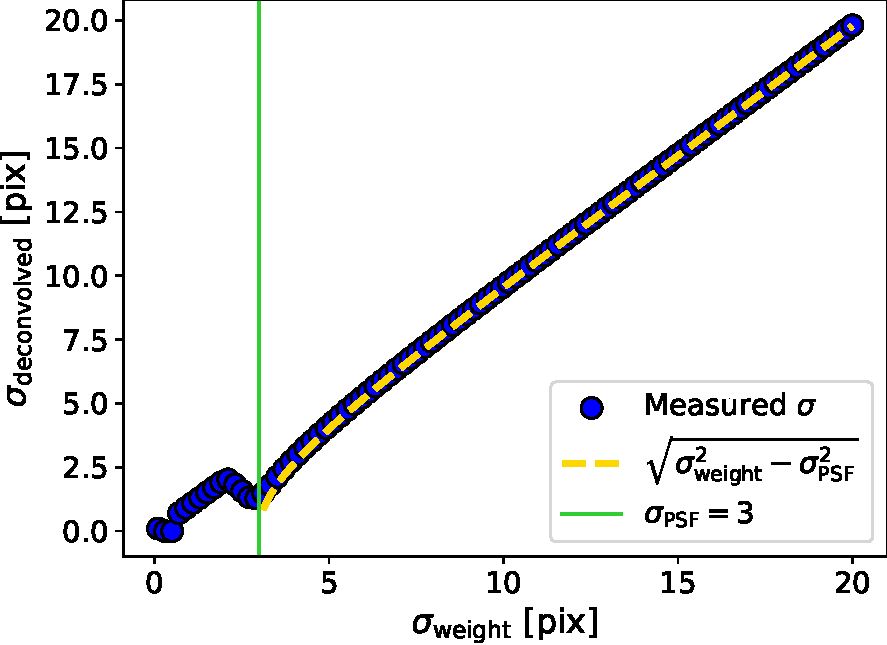
\includegraphics[width=0.7\linewidth]{results/figures/simulation/deconvolution_relation.pdf}
    \caption{Relation between the size of the weight function after deconvolution and the size before deconvolution. The deconvolution follows the theoretical relation for the weight functions that are larger than the \gls{psf}, but starts to fail when the weight function is similar in size to or smaller than the \gls{psf}. }
    \label{fig: deconvolution}
\end{figure}
The measured size of the deconvolved weight function aligns well with the expected result for weight sizes that are larger than the \gls{psf}. When the size of the weight function comes close to the size of the \gls{psf}, the results start to deviate slightly from the theoretical value, and when the weight function is smaller than the \gls{psf}, the deconvolution starts to fail. 

\begin{figure}[H]
    \centering
    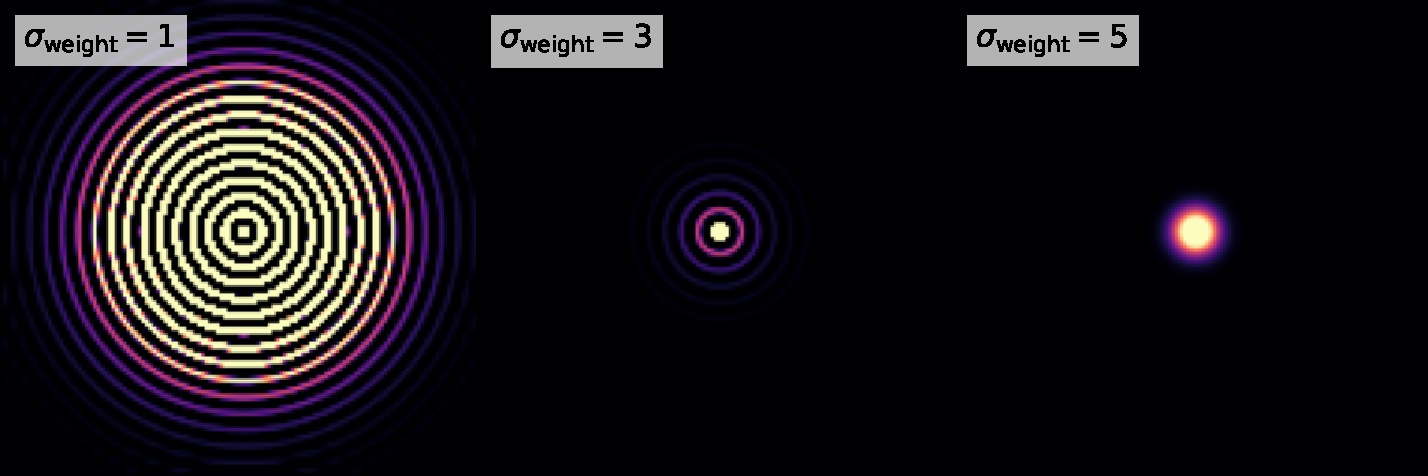
\includegraphics[width=0.9\linewidth]{results/figures/simulation/2_regimes.pdf}
    \caption{The three regimes of the deconvolution of a Gaussian weight function by a Gaussian \gls{psf}. The case where the weight function is smaller than the \gls{psf} (Left). The case where the weight function is the same size as the \gls{psf} (middle). The case where the weight function is larger than the \gls{psf}, and deconvolves correctly (right).}
    \label{fig: 2 regimes}
\end{figure}
\autoref{fig: 2 regimes} shows that when the weight function is smaller than the \gls{psf}, the resulting deconvolved weight function has ringing artifacts in it. This is due to the amplification of higher-frequency modes in the deconvolution.  Even when the weight function is the same size as the \gls{psf}, there are still some of these effects. However, in the case that the weight function is bigger than the \gls{psf}, it deconvolves to the correct Gaussian shape. 


\subsection{Flux Accuracy}\label{subsec: result flux accuracy}

The \gls{x-bap} method is applied to the simulated observation to assess its effectiveness. First, the method is applied to different locations in the observation, and the result is compared to the true flux at that location. This is done to both look at the accuracy of the method as well as the accuracy of the translation of the weight function by multiplying it with a complex factor in Fourier space, as described in \Cref{subsec: applying pca-phot algorithm}.

\begin{figure}[H]
    \centering
    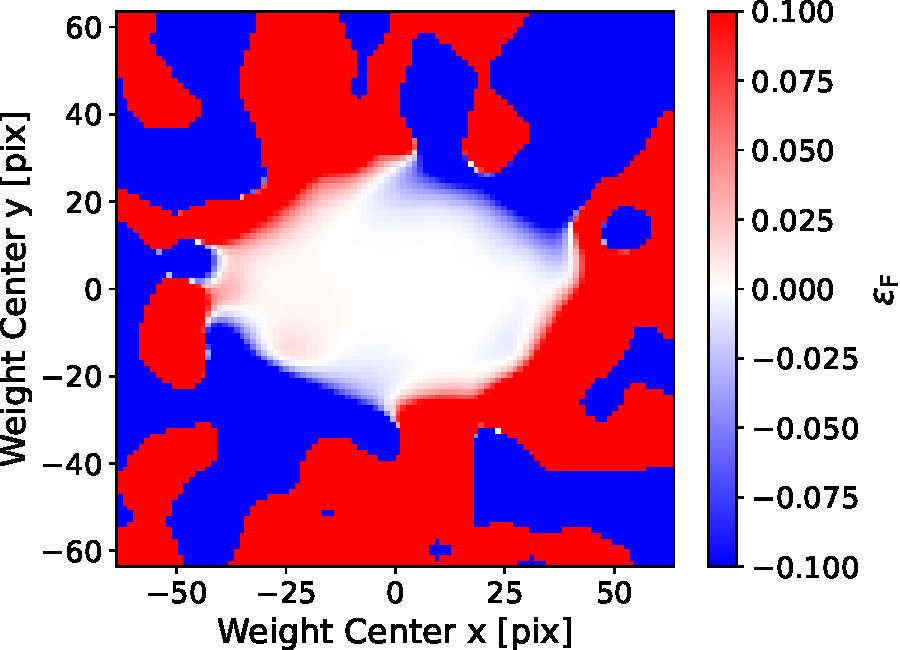
\includegraphics[width=0.7\linewidth]{results/figures/simulation/center_accuracy.pdf}
    \caption{The fractional error on the measured flux compared to the true flux at different positions in the simulated image. The yellow line denotes the border of 1$\%$ absolute error. The measured flux is most accurate near the center of the image, i.e., the galaxy. Further from the center, the flux measurements are less accurate due to the effects of the noise in the observation.}
    \label{fig: center accuracy}
\end{figure}
The flux measurements are accurate near the center of the simulated observation where the simulated galaxy resides. Further outwards, the measurements become less accurate as these regions are dominated by noise. There seem to be no artifacts due to the translation of the weight function in real space by multiplying the Fourier transform by a complex factor based on the shift in real space. This allows for an analytical weight function, whereas with interpolation the weight function is only an approximation of the true weight function. In case a different method, such as interpolation, is used to find the post-seeing weight function on a subgrid level, this would introduce grid-like artifacts in \autoref{fig: center accuracy}.

The effectiveness of the \gls{x-bap} method is tested for different combinations of the weight size and the size of the \gls{psf}. The measured flux values are compared to the true flux values, where the weight function is centered at the middle of the image, i.e., the galaxy.

\begin{figure}[H]
    \centering
    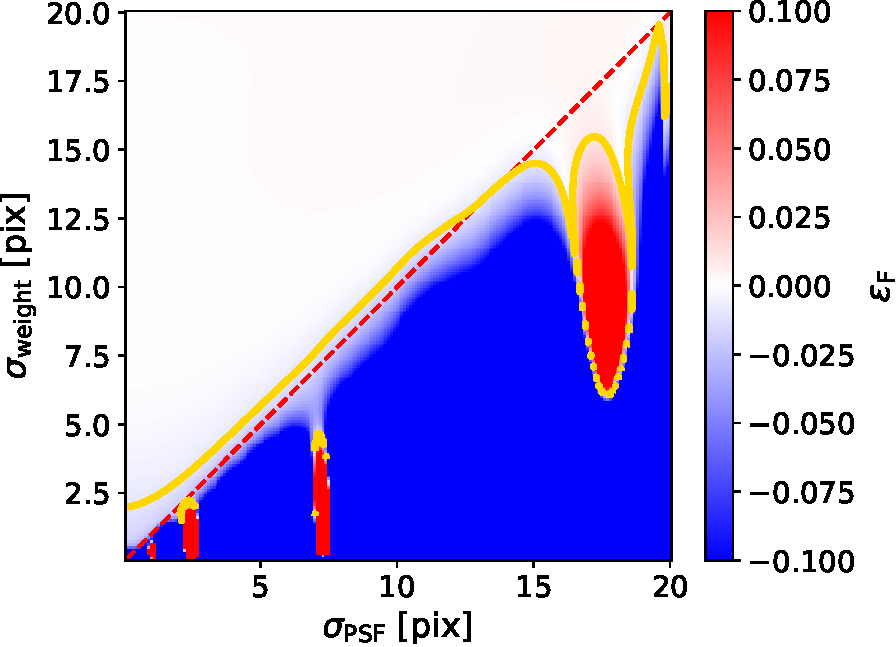
\includegraphics[width=0.7\linewidth]{results/figures/simulation/flux_accuracy.pdf}
    \caption{The fractional error on the measured flux compared to the true flux for different combinations of weights and \gls{psf} sizes. The solid yellow line denotes the border of 1$\%$ relative error, and the dashed red line shows where the weight function and the \gls{psf} have the same size. The measured flux is accurate when the weight function is bigger than the \gls{psf}. However, the measurements become unstable when the weight function is smaller than the \gls{psf}.}
    \label{fig: flux accuracy}
\end{figure}
\autoref{fig: flux accuracy} shows two different regimes. The first region is the measurements taken with weights smaller than the \gls{psf}, where the measured flux values are inaccurate. This result is expected as the deconvolution of the weight function, where the \gls{psf} is larger, results in artifacts, as shown in \Cref{subsec: Deconvolution}. In the region where the weight function is larger than the \gls{psf}, the flux measurements are accurate. This result means that there is no inherent bias in the method within the tested parameters.


\subsection{Flux Error Accuracy}\label{subsec: flux error accuracy}

10000 different observations are simulated with different instances of noise, and the flux and error on the flux are estimated from these observations. The standard deviation of the flux is compared to the mean of the predicted standard deviation of the flux. First, the errors are calculated using the background noise to estimate the error on the flux (as described in \Cref{subsec: Noise Estimation from background Noise}. Thereafter, the errors are calculated using the \gls{rms} map to estimate the error on the flux (as described in \Cref{subsec: Noise from RMS}.

\subsubsection{Error from Background Noise}

\begin{figure}[H]
    \centering
    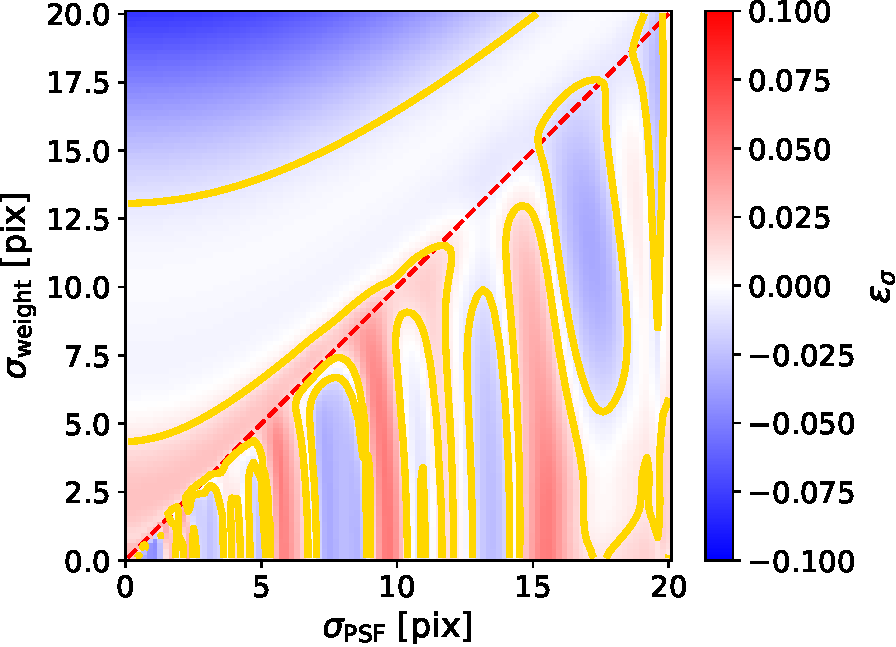
\includegraphics[width=0.7\linewidth]{results/figures/simulation/sigma_accuracy.pdf}
    \caption{The measured error divided by the true flux error, computed from the distribution of flux values across different noise instances. The error in the flux is measured using the background noise. The yellow solid line denotes the border of 1\%. The PSF size and weight do not affect the accuracy of the error.}
    \label{fig: background error PSF}
\end{figure}
The relative error on the standard deviation shown in \autoref{fig: background error PSF} indicates that the estimated error is accurate and does not depend on the PSF size or the weight. Especially, in the region above the red line where the deconvolution is stable, as discussed in \Cref{subsec: result flux accuracy}.

\begin{figure}[H]
    \centering
    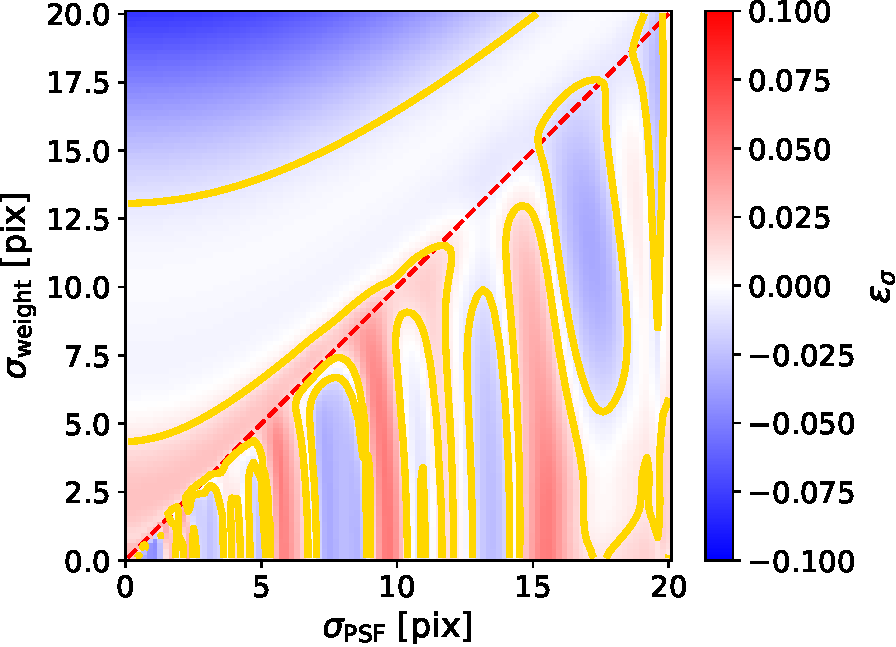
\includegraphics[width=0.7\linewidth]{results/figures/simulation/sigma_accuracy.pdf}
    \caption{The measured error divided by the true flux error, computed from the distribution of flux values across different noise instances. The error in the flux is measured using the background noise. The yellow solid line denotes the border of 1\%. The PSF size and weight do not affect the accuracy of the error.}
    \label{fig: correlated noise background}
\end{figure}


\subsubsection{Error from RMS Map}

\begin{figure}[H]
    \centering
    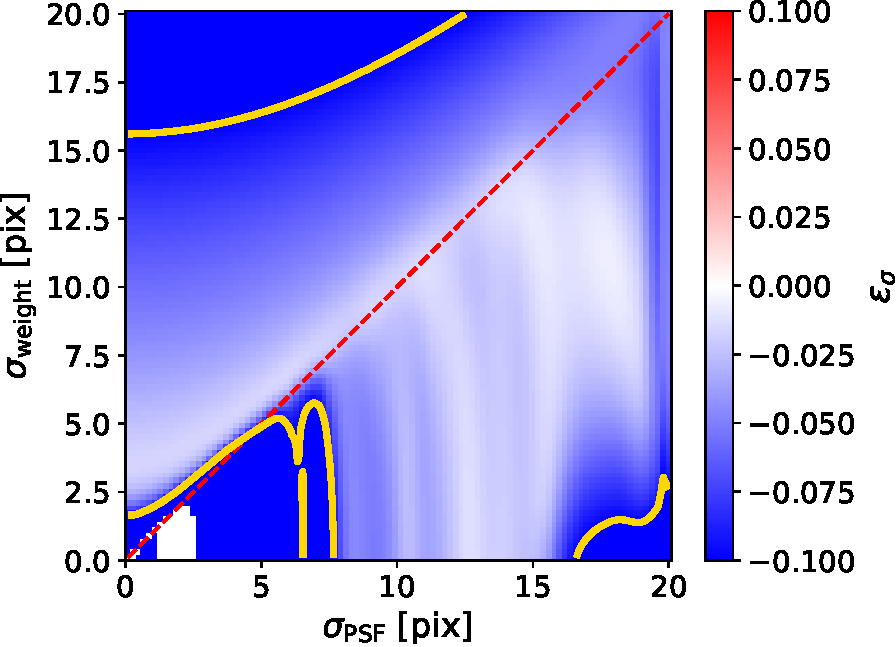
\includegraphics[width=0.7\linewidth]{results/figures/simulation/rms_accuracy.pdf}
    \caption{The measured error divided by the true flux error, computed from the distribution of flux values across different noise instances. The error in the flux is measured using the \gls{rms} and the correlation function derived from the background noise. The yellow solid line denotes the border of 1\%. The PSF size and weight do not affect the accuracy of the error.}
    \label{fig: rms error PSF}
\end{figure}
The relative error on the standard deviation shown in \autoref{fig: rms error PSF} indicates that the estimated error is accurate and does not depend on the PSF size or the weight. This result is similar to the result from \autoref{fig: background error PSF}, where the results are also largely accurate in the region above the red line, but start to underestimate the noise for the case where the weight function is large. 

\begin{figure}[H]
    \centering
    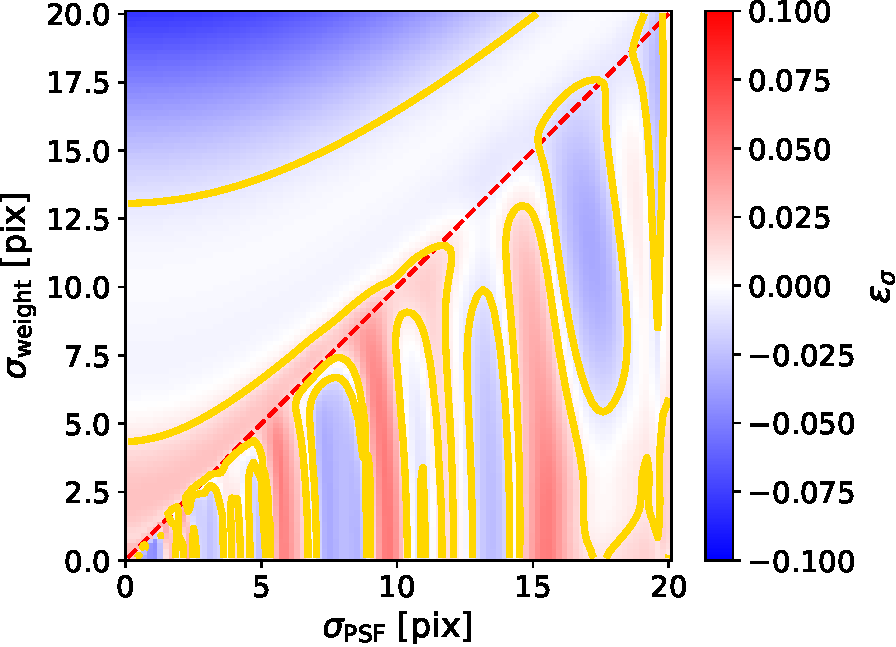
\includegraphics[width=0.7\linewidth]{results/figures/simulation/sigma_accuracy.pdf}
    \caption{The measured error divided by the true flux error, computed from the distribution of flux values across different noise instances. The error in the flux is measured using the background noise. The yellow solid line denotes the border of 1\%. The PSF size and weight do not affect the accuracy of the error.}
    \label{fig: correlated noise rms}
\end{figure}


\subsection{PSF shape}

In the previous subsections, the \gls{psf} used for the deconvolution of the weight function was exactly the same as the \gls{psf} used to generate the images. However, in real observations, this is unlikely to be the case. To examine this, the flux measurements for different combinations of the Gaussian \gls{psf} used for the generation of the simulated observation and the Gaussian \gls{psf} used for the deconvolution are compared. For this, a weight function with a scale parameter of 20 pixels is used.

\begin{figure}[H]
    \centering
    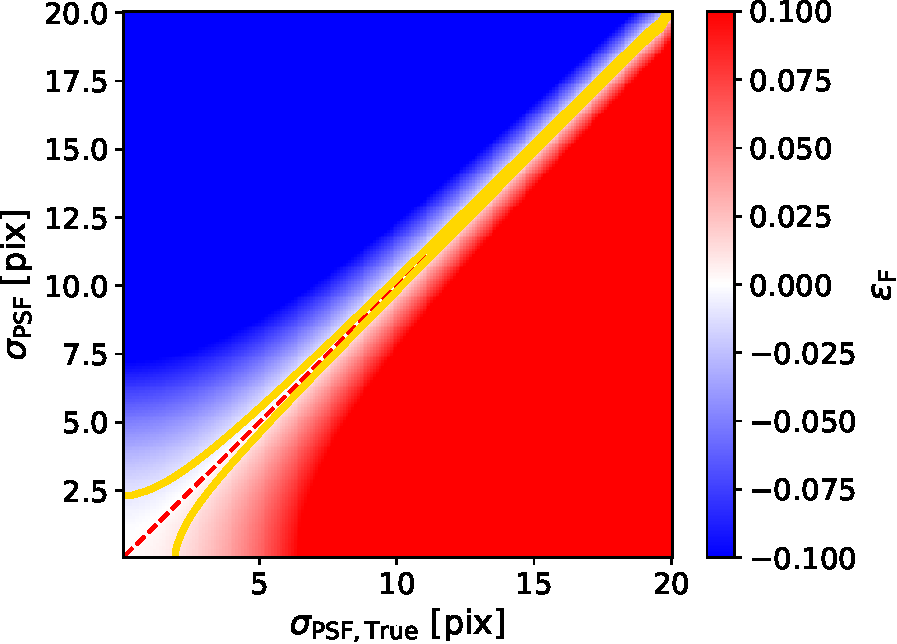
\includegraphics[width=0.7\linewidth]{results/figures/simulation/psf_dependence.pdf}
    \caption{The relative error on the flux for different combinations of the \gls{psf} used for the deconvolution and the \gls{psf} used to generate the observation. When the \gls{psf} used for the deconvolution is larger than the \gls{psf} used for the generation of the observation, the flux is underestimated. The reverse is true when the \gls{psf} used for the deconvolution is smaller than the \gls{psf} used for the generation of the observation. }
    \label{fig: psf shape}
\end{figure}
\autoref{fig: psf shape} shows that the \gls{psf} used for the deconvolution must be close to the \gls{psf} used for the generation of the observation to give the most accurate results for the measurements of the flux. In the case that the \gls{psf} for the generation of the observation becomes large, the \gls{psf} used for the deconvolution has to be closer to the size of the true \gls{psf} to achieve the same accuracy. The difference in sign based on whether the \gls{psf} is bigger or smaller than the true \gls{psf} comes from the resulting size of the post-seeing weight function. When the \gls{psf} used for the deconvolution is greater than the true \gls{psf}, the post-seeing weight function becomes smaller than it should be resulting in a smaller amount of aperture flux measrued. The inverse is true in the case that the \gls{psf} used for the deconvolution is smaller than the true \gls{psf}. 
\textbf{include figure explaining this?}

\subsection{Aperture Shape}

The shape of the weight function also affects the measured flux and the error in the measurement. In this section, the shape and the size of the weight function are varied both in the x- and the y-direction, without rotating the weight function. 

\begin{figure}[H]
    \centering
    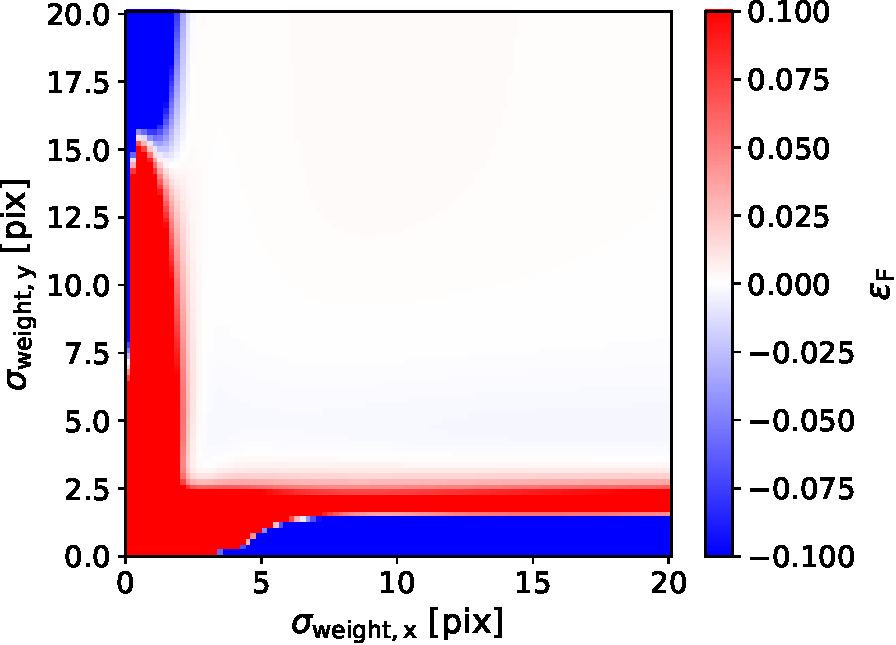
\includegraphics[width=0.7\linewidth]{results/figures/simulation/weight_accuracy.pdf}
    \caption{The relative error on the flux measurement for different shapes of the weight function. The error is close to 0 when the size of the weight function is larger than the size of the \gls{psf} in both directions.}
    \label{fig: weight accuracy}
\end{figure}
The flux measurement of the elliptical weight function is accurate, as shown in \autoref{fig: weight accuracy}, as long as the scale parameter in both directions is larger than the size of the \gls{psf}, which is expected following the results from \autoref{subsec: result flux accuracy}. When measuring the flux from a source, getting a high \gls{snr} is important to get the most accurate results. 

\begin{figure}[H]
    \centering
    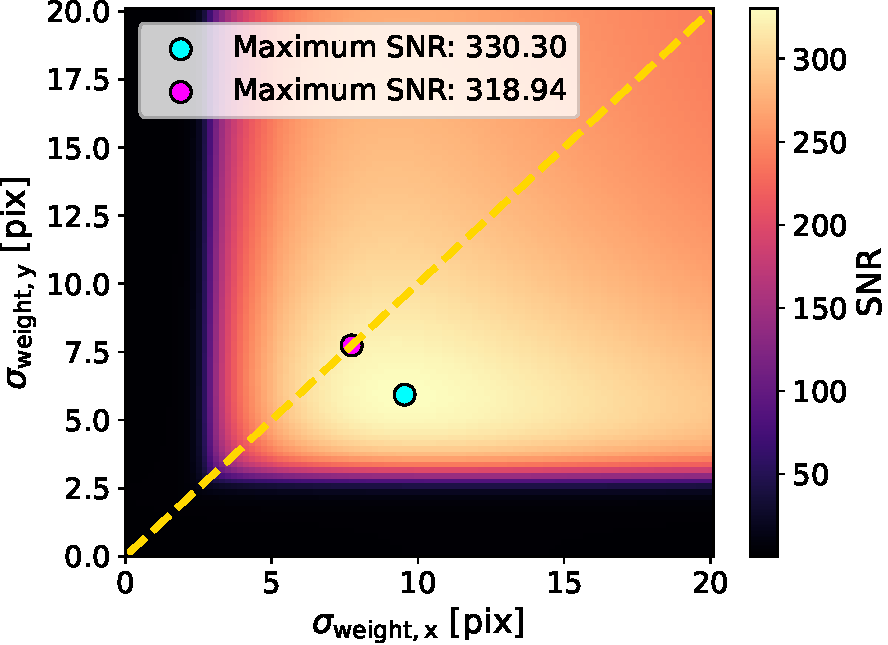
\includegraphics[width=0.7\linewidth]{results/figures/simulation/weight_size_snr.pdf}
    \caption{The \gls{snr} for different combinations of the horizontal and vertical standard deviations of the weight. The dashed line shows the spherical Gaussians; all the off-diagonal combinations are elliptical weights.}
    \label{fig: best aperture}
\end{figure}
The maximum \gls{snr} of a circular Gaussian weight function (diagonal line) in \autoref{fig: best aperture} is slightly lower than the \gls{snr} compared to the maximum \gls{snr} for the elliptical Gaussian weight functions. Therefore, the size can be optimized to give a higher \gls{snr} for each source in an image. However, there is a computational disadvantage to this, as such an elliptical Gaussian weight function requires 3 parameters; it is unlikely that different sources have the same weight function that optimizes the \gls{snr}, whereas circular Gaussian weight functions only require 1 parameter, so more of the deconvolved weight functions can be used for different sources. Another problem that arises from the fact that there are 3 parameters is that the extra free parameters allow for overfitting. For example, when there is a bright source close to the target, the weight function that optimizes the \gls{snr} gives more weight to the bright source. This results in the measured flux not representing the flux of the target. The gain of the signal using an elliptical weight is relatively small

% \subsection{Summary of simulation results}


\newpage